\section{Experiments}
\label{sec:experiments}

We evaluate four questions: (Q1) Does the structured head preserve ordinary VLA competence? (Q2) Do executable clauses improve long-horizon execution, and does the spline head benefit more? (Q3) Does changing a clause change the corresponding behavior? (Q4) Does separating shape and time enable useful deployment control?

\subsection{Setup}

\textbf{Policies.} All policies use the 450M-parameter SmolVLA backbone \cite{shukor2025smolvla}. We compare \textbf{A}, stock 50-waypoint SmolVLA; \textbf{B}, eight-control-point cubic splines over a fixed 20-step window; and \textbf{C}, our event-aligned spline with learned duration. A and C are the matched heads in language experiments. Unless noted, policies execute 10 actions before replanning. Training seeds vary both optimization and action-expert initialization.

\textbf{Training.} The broad LIBERO comparison trains every head for 100,000 updates with batch size 32 on the identical 40-task dataset, using seeds 1000--1002 and the same pretrained SmolVLM initialization. The clause factorial starts from the corresponding 100k A or C checkpoint and applies 7,500 matched updates (batch 32) to one frozen 71-episode manifest. RoboCasa label comparisons likewise hold initialization, physical episodes, update count, and optimizer schedule fixed within each seed. All timing and rate variants are configuration-only decodes of an already trained checkpoint unless explicitly labeled as a language or retrained baseline.

\textbf{Domains and metrics.} LIBERO \cite{liu2023libero} supplies four ten-task suites and the two multi-object LIBERO-Long tasks used for the clause factorial. We report task success. CALVIN \cite{mees2022calvin} uses the official five-instruction chain protocol; its metric is the mean number of consecutive tasks completed. RoboCasa365 \cite{nasiriany2026robocasa365} tests mobile manipulation in diverse kitchens. Paired comparisons use identical initial simulator states and policy seeds. Exact-replay gates hash initial observations, simulator states, prompts, and complete action traces; all 30 clause-study gates passed across 6,000 control and treatment rollouts.

\subsection{Q1: Broad Competence Is Preserved}

Table~\ref{tab:libero} reports three training seeds and 1,200 rollouts per arm across four suites (300 per suite). A Barnard test with Bonferroni correction finds no significant arm difference after protocol crossing. C is within 1.4 points of waypoint SmolVLA overall and has the lowest across-seed variation, so the new interface does not purchase its downstream capabilities by sacrificing broad success.

\begin{table}[t]
\centering
\caption{LIBERO success (\%, three training seeds). ``Avg.'' averages the four suites; $\pm$ is its seed standard deviation.}
\label{tab:libero}
\setlength{\tabcolsep}{3.5pt}
\begin{tabular}{lrrrrrr}
\toprule
Head & Obj. & Spatial & Goal & Long & Avg. & SD \\
\midrule
A Waypoint & 94.7 & 84.3 & 86.0 & 63.3 & \textbf{82.1} & 1.8 \\
B Fixed spline & \textbf{96.3} & 77.7 & 84.0 & \textbf{65.3} & 80.8 & 2.5 \\
C Spline+duration & 92.3 & 77.3 & \textbf{89.3} & 63.7 & 80.7 & \textbf{1.3} \\
\bottomrule
\end{tabular}
\end{table}

\begin{figure*}[t]
    \centering
    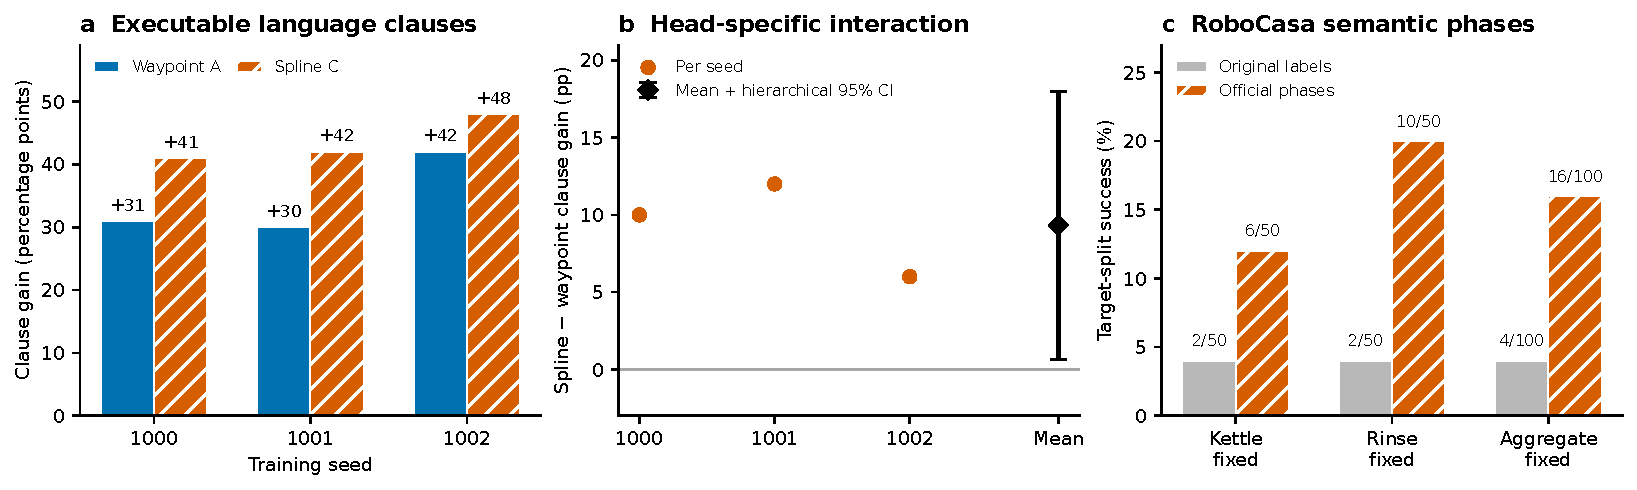
\includegraphics[width=\textwidth]{figures/headline_results.pdf}
    \caption{\textbf{Executable-language results.} (a) Clauses improve both heads on two LIBERO-Long tasks and all training seeds. (b) Their gain is consistently larger for the event-aligned spline head; the hierarchical interval excludes zero. (c) Official semantic phases improve the first-seed RoboCasa365 target split. The independent-seed replication appears in Table~\ref{tab:robocasa}.}
    \label{fig:headline}
\end{figure*}

\subsection{Q2: Executable Clauses Improve Long-Horizon Tasks}

An initial Molmo-2 segment-label pilot moved t0 from 24/50 to 38/50 while leaving the ten-task suite approximately flat; it motivated a cleaner exact-clause intervention.

The controlled study contains 33 demonstrations of LIBERO-Long t0 (soup and tomato into a basket) and 38 of t4 (two mugs onto different plates): 71 episodes and 19,378 frames total. Whole-caption and clause datasets are byte-identical in every non-language column. Within each head, the two language treatments receive the same head-matched 100k-step warm start, episodes, batch size, and 7,500-step budget.

Figure~\ref{fig:headline}a shows the aggregate result over 50 states per task. Pooled across seeds, A rises from 7.0\% to 41.3\% and C from 11.7\% to 55.3\%. Clauses improve A by 31, 30, and 42~pp across seeds and C by 41, 42, and 48~pp. The mean gains are 34.33 and 43.67~pp, respectively. The difference-in-differences,
\begin{equation}
  \Delta_{\mathrm{head}}=(C_{\mathrm{clause}}-C_{\mathrm{whole}})
       -(A_{\mathrm{clause}}-A_{\mathrm{whole}}),
\end{equation}
is +10, +12, and +6~pp (mean +9.33~pp). A hierarchical bootstrap over training seeds and paired states gives a 95\% CI of 0.67--18.0~pp; the seed-level $t$ interval is 1.74--16.92~pp. This establishes an action-representation interaction, not merely an advantage from adding labels.

Two controls isolate execution from relabeling. First, clause-trained policies evaluated once with a static compound prompt regress by 9.33~pp (A) and 24.0~pp (C) relative to their original-label counterparts. Second, advancing C on its predicted close-to-open gripper event retains a 40.33~pp mean clause gain, comparable to the matched fixed-clock gain. Clause-conditioned C also succeeds faster descriptively on seed 1000 (median steps t0, 321$\rightarrow$270; t4, 292$\rightarrow$236).

\subsection{Q3: Language Changes the Requested Behavior}

We reverse the two clauses and score which official goal predicate is reached first. A privileged predicate transition advances the program in this diagnostic only. On t4, both A and C change the first completed object in the requested direction on 10/50 paired states, with zero opposite-direction changes (two-sided sign test $p=.00195$). Of 12 states with a unique first goal under both orders, 10 flip as requested. Final conjunction success falls from 49/100 to 16/100 for A and from 55/100 to 21/100 for C: language can redirect the first subgoal, but canonical-order bias still impairs retention and completion. This distinction prevents first-subgoal steering from being mistaken for solved compositional generalization.

\subsection{RoboCasa365 Semantic Phases}

RoboCasa's longer manipulation sequences test whether short language units remain useful beyond LIBERO. We relabel identical physical demonstrations using the benchmark's official semantic phases: pick, place, and actuate for KettleBoiling; faucet and basin-washing phases for RinseSinkBasin. Policies use an outcome-independent fixed phase clock. Table~\ref{tab:robocasa} shows that the two-task aggregate improves on both training seeds. Rinse replicates strongly; Kettle is heterogeneous.

\begin{table}[t]
\centering
\caption{RoboCasa365 target-split full-task success. Each cell is original labels $\rightarrow$ official phase labels.}
\label{tab:robocasa}
\setlength{\tabcolsep}{4pt}
\begin{tabular}{crrr}
\toprule
Seed & Kettle & Rinse & Aggregate \\
\midrule
1000 & 2/50$\rightarrow$6/50 & 2/50$\rightarrow$\textbf{10/50} & 4/100$\rightarrow$\textbf{16/100} \\
1001 & 2/20$\rightarrow$1/20 & 1/20$\rightarrow$\textbf{8/20} & 3/40$\rightarrow$\textbf{9/40} \\
\bottomrule
\end{tabular}
\end{table}

The aggregate gains are +12 and +15~pp (4$\times$ and 3$\times$ the original counts), for an unweighted mean gain of 13.5~pp. On seed 1000, phase labels increase Kettle grasps from 24/50 to 39/50 ($p=.00346$) and Rinse rollouts reaching water-on/one washed region from 7/50 to 22/50 ($p=.00175$). The latter mechanism replicates 3/20$\rightarrow$12/20 on seed 1001 ($p=.00791$). Figure~\ref{fig:kettle} localizes a matched Kettle outcome: both policies grasp and place from the same initial state, but only phase supervision preserves progress through burner actuation.

\begin{figure*}[t]
    \centering
    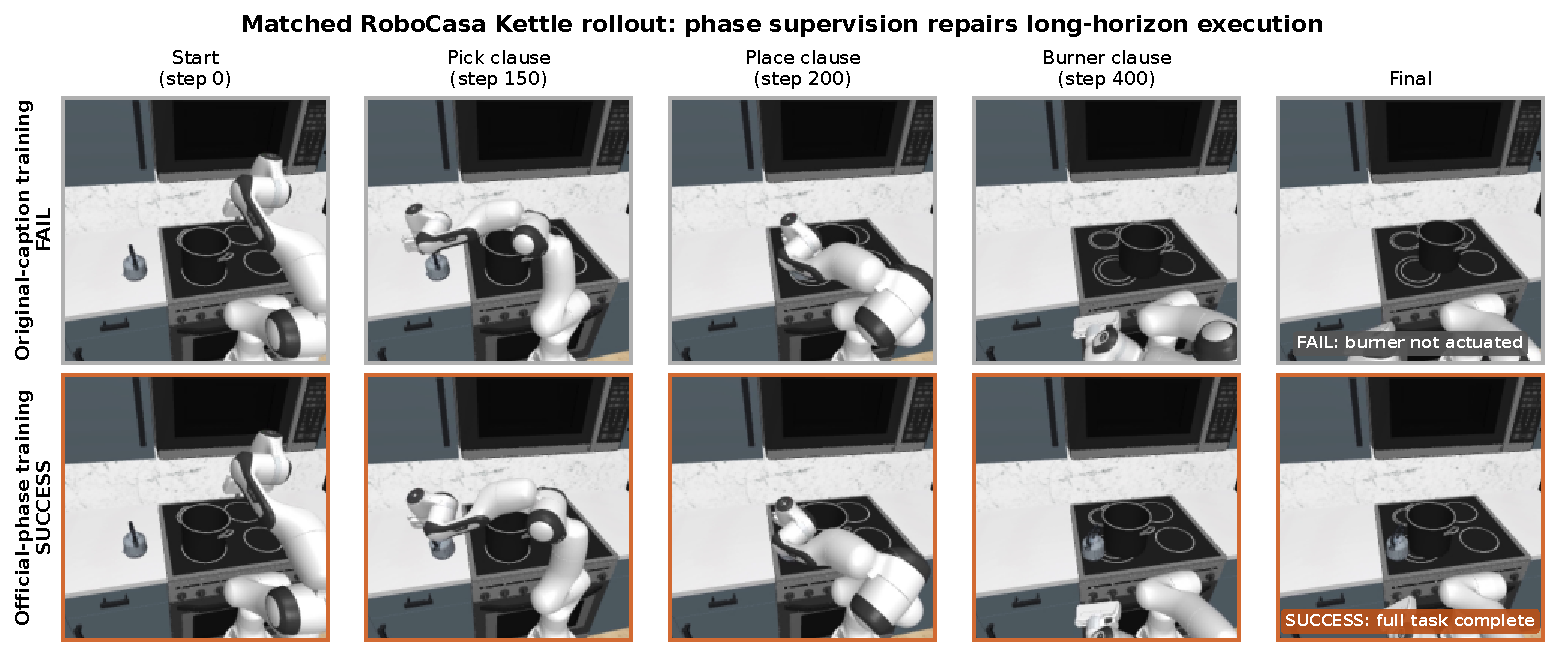
\includegraphics[width=\textwidth]{figures/kettle_phase_storyboard.pdf}
    \caption{\textbf{Matched RoboCasa365 Kettle rollout.} The original-caption and official-phase policies share the exact initial observation. Both reach grasp and stove contact at similar times; only the phase-trained policy completes burner actuation (516 steps versus failure at the 1,500-step limit).}
    \label{fig:kettle}
\end{figure*}

Wrong-instruction controls confirm prompt sensitivity in atomic tasks: changing drawer left$\leftrightarrow$right reduces A/C success from 7/50 and 6/50 to zero; rack in$\leftrightarrow$out reduces 18/50 and 15/50 to zero. Since the reward still scores the original goal, these controls establish suppression of an incompatible behavior, not alternate-goal completion.

\subsection{Q4: The Learned Physical Clock Is Controllable}

The duration head predicts held-out event times with 1.61-step MAE and Pearson $r=.819$; event-versus-cap balanced accuracy is .892. Figure~\ref{fig:control} reports absolute outcomes before paired differences so that every gain has an explicit comparator. On CALVIN, waypoint A averages 1.56 completed tasks, unretimed C averages 1.31, and uniformly retimed C averages 1.69. Every C seed improves under the same decode-only intervention. The paired gain over C-base is 0.379 (95\% CI, 0.318--0.441) at 1.42$\times$ realized speed; retimed C also exceeds waypoint A by 0.127 (CI, 0.063--0.191) while matching first-task success (69.9\% versus 69.4\%, McNemar $p=.56$). Both contrasts pool three seeds and 1,000 identical official chains per seed.

\begin{figure*}[t]
    \centering
    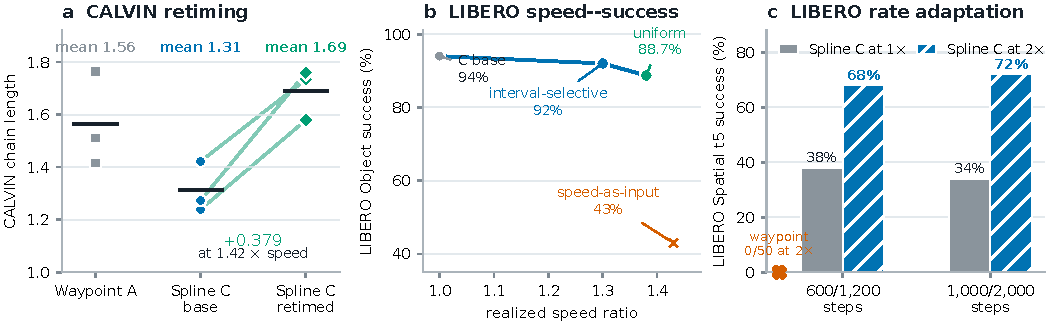
\includegraphics[width=\textwidth]{figures/control_results.pdf}
    \caption{\textbf{Timing and control-rate results.} (a) Absolute CALVIN chain length for three training seeds; horizontal ticks are means and lines connect each C-base seed to its retimed counterpart. Uniform retiming recovers the unretimed spline deficit and exceeds waypoint A while executing faster. (b) On LIBERO Object, the same C checkpoint traces a speed--success frontier; the separately retrained speed-as-input baseline collapses near the same speed. (c) Sampling the same spline at twice the control rate repairs LIBERO Spatial t5 under two independently budgeted horizon protocols; direct waypoint replay fails on the measured $2\times$ condition.}
    \label{fig:control}
\end{figure*}

The LIBERO panels separate two uses of time. Retiming changes how quickly normalized phase is traversed: interval-selective compression retains 92\% success at 1.30$\times$, versus 94\% for C-base, while uniform compression reaches 1.38$\times$ at 88.7\%. A budget-matched speed-as-input policy requires retraining yet reaches only 43\% at 1.43$\times$. Rate adaptation instead samples the same curve more densely. At $2\times$ control rate, C improves from 38\% to 68\% and from 34\% to 72\% under two paired horizon protocols; direct waypoint replay is 0/50. The gain is task-selective---the full Spatial suite remains approximately flat---and is therefore a remedy for tracking-limited cells, not a universal success boost.

\begin{table*}[t]
\centering
\caption{Additional uses of the learned spline interface. Each row states what changes relative to the named baseline; $\dagger$ marks a supporting single-seed mechanism cell rather than a headline aggregate.}
\label{tab:control}
\small
\setlength{\tabcolsep}{4pt}
\renewcommand{\arraystretch}{1.08}
\begin{tabularx}{\textwidth}{@{}l X X l@{}}
\toprule
Use & Intervention and comparator & Audited outcome & Evaluation \\
\midrule
Language pace & CALVIN prompt: plain $\leftrightarrow$ ``quickly'' / ``slowly'' & Realized pace $+16\%/-16\%$; plain \mbox{$1.382\rightarrow1.553$} with ``quickly'' ($\Delta=.172$, $p=.018$; Bonferroni $p=.035$) & 600 paired chains/condition \\
Event replanning & Fixed cadence $\rightarrow$ replan at $\hat T-4$ & Matched success with $2.7\times$ fewer policy calls on LIBERO and $2.1\times$ fewer on CALVIN & fixed checkpoints; CALVIN $3\times1{,}000$ \\
Feasibility stretch$\dagger$ & Clip coarse-rate deltas $\rightarrow$ lengthen the execution window until feasible & $+19$ success points at half control rate & paired LIBERO cell \\
Shape capacity$\dagger$ & Long t7: eight $\rightarrow$ twelve control points & 42\%$\rightarrow$78\% success & paired LIBERO cell \\
Execution cadence$\dagger$ & Long t8: same n16/h48 checkpoint, short $\rightarrow$ long execution & 30\%$\rightarrow$52\% success & paired LIBERO cell \\
Failure signal & Threshold a stalled $\hat T$ countdown & 86\% precision / 52\% recall & fixed LIBERO checkpoint \\
Contact ease-out & Linear phase $\rightarrow$ endpoint-preserving cosine warp & Terminal velocity $0.14\times$ with identical endpoint & offline kinematics \\
Compute & Waypoint A $\rightarrow$ spline C policy call & 209.1$\rightarrow$221.7~ms (+6\%); precomputed spline decode $<1$~ms & A40 latency \\
\bottomrule
\end{tabularx}
\end{table*}

Retiming is data-dependent rather than universally beneficial. An imitation policy inherits the demonstrator's time map; compression can harvest dead time, but it can also induce actuator clipping or rush precision-critical contact. Scripted LIBERO contains little removable hesitation, so interval-selective warping loses the least. CALVIN demonstrations contain distributed low-speed dithering, so uniform retiming removes more harmful hesitation and is best. RoboCasa operates near its action bound (38\% of frames exceed 60\% of the bound), so aggressive compression is clipped or re-expanded and becomes success-neutral. Nevertheless, successful Kettle rollouts shorten descriptively from 230 to 97 steps. These measured regimes explain why one decode rule should not be expected to dominate every dataset.

The interface remains efficient because the VLM dominates latency. An A40 policy call increases only 6\% from A to C (Table~\ref{tab:control}); at $2\times$ rate, curve resampling yields twice as many environment steps without an additional neural query. With fixed flow-matching noise, decoding the same tokens at $1\times$ and $2\times$ has approximately zero endpoint/path deviation from the fine reference, while commanded jerk falls from .040 to .0055. Event-scheduled replanning then uses the learned clock to reduce policy calls, rather than merely increasing low-cost interpolation steps.

\subsection{Real-Robot Evaluation}
\label{sec:hardware}

\textit{Protocol frozen; quantitative trials are being collected.} The platform contains two 7-DoF xArm7 manipulators on 1-DoF linear rails, with one arm providing an external camera view and the other executing gripper actions. Demonstrations are collected with a handheld one-arm teleoperation device. Existing 3D-printed fixtures support two focused programs: (i) open drawer $\rightarrow$ insert object $\rightarrow$ close or leave open, enabling a matched late-clause intervention with an identical prefix; and (ii) a physically valid non-cuboid stacking order. The rail remains fixed unless reach requires it.

We will derive whole-caption and clause-labeled datasets from the same physical trajectories and compare A/C$\times$whole/clause whenever all four policies pass seen-program competence. Evaluation uses 20 frozen initial configurations per condition, interleaved treatment order, and reports requested first subgoal, final success, and prefix-versus-late trajectory divergence. A filmstrip and result table will replace this paragraph after the frozen evaluation; no hardware result is assumed in the claims above.
